\documentclass[11pt,a4paper,oldfontcommands,openany]{memoir}
\usepackage{graphicx}
\usepackage[]{color}
\usepackage{courier}
\usepackage[usenames,dvipsnames]{xcolor}
\usepackage[breakable, theorems, skins]{tcolorbox}
\usepackage[]{media9}
\usepackage{lipsum}
\tcbset{enhanced}
%% maxwidth is the original width if it is less than linewidth
%% otherwise use linewidth (to make sure the graphics do not exceed the margin)
\makeatletter
\def\maxwidth{ %
  \ifdim\Gin@nat@width>\linewidth
    \linewidth
  \else
    \Gin@nat@width
  \fi
}
\makeatother

\DeclareRobustCommand{\mybox}[2][gray!15]{%
\begin{tcolorbox}[   %% Adjust the following parameters at will.
        breakable,
        left=0pt,
        right=0pt,
        top=0pt,
        bottom=0pt,
        colback=#1,
        colframe=#1,
        width=\dimexpr\textwidth\relax, 
        enlarge left by=0mm,
        boxsep=5pt,
        arc=0pt,outer arc=0pt,
        ]
        #2
\end{tcolorbox}
}


\definecolor{fgcolor}{rgb}{0.345, 0.345, 0.345}
\newcommand{\hlnum}[1]{\textcolor[rgb]{0.686,0.059,0.569}{#1}}%
\newcommand{\hlstr}[1]{\textcolor[rgb]{0.192,0.494,0.8}{#1}}%
\newcommand{\hlcom}[1]{\textcolor[rgb]{0.678,0.584,0.686}{\textit{#1}}}%
\newcommand{\hlopt}[1]{\textcolor[rgb]{0,0,0}{#1}}%
\newcommand{\hlstd}[1]{\textcolor[rgb]{0.345,0.345,0.345}{#1}}%
\newcommand{\hlkwa}[1]{\textcolor[rgb]{0.161,0.373,0.58}{\textbf{#1}}}%
\newcommand{\hlkwb}[1]{\textcolor[rgb]{0.69,0.353,0.396}{#1}}%
\newcommand{\hlkwc}[1]{\textcolor[rgb]{0.333,0.667,0.333}{#1}}%
\newcommand{\hlkwd}[1]{\textcolor[rgb]{0.737,0.353,0.396}{\textbf{#1}}}%

\usepackage{framed}
\makeatletter
\newenvironment{kframe}{%
 \def\at@end@of@kframe{}%
 \ifinner\ifhmode%
  \def\at@end@of@kframe{\end{minipage}}%
  \begin{minipage}{\columnwidth}%
 \fi\fi%
 \def\FrameCommand##1{\hskip\@totalleftmargin \hskip-\fboxsep
 \colorbox{shadecolor}{##1}\hskip-\fboxsep
     % There is no \\@totalrightmargin, so:
     \hskip-\linewidth \hskip-\@totalleftmargin \hskip\columnwidth}%
 \MakeFramed {\advance\hsize-\width
   \@totalleftmargin\z@ \linewidth\hsize
   \@setminipage}}%
 {\par\unskip\endMakeFramed%
 \at@end@of@kframe}
\makeatother

\definecolor{shadecolor}{rgb}{.97, .97, .97}
\definecolor{messagecolor}{rgb}{0, 0, 0}
\definecolor{warningcolor}{rgb}{1, 0, 1}
\definecolor{errorcolor}{rgb}{1, 0, 0}
\newenvironment{knitrout}{}{} % an empty environment to be redefined in TeX

\usepackage{alltt}
\setlength{\parindent}{0pt} % Remove indent at new paragraphs
\setcounter{secnumdepth}{4}  % Remove section numbering at certain depth # If zero, then no numbering of sections
\setcounter{tocdepth}{4} % Determines number of subsections that will have tabs
\usepackage{tabu}
\usepackage{url}

\usepackage[round]{natbib}   % omit 'round' option if you prefer square brackets
\bibliographystyle{plainnat}

\usepackage{fixltx2e}
%\usepackage{graphicx}	% For external pictures
\usepackage{float}
\usepackage{subfig}	% Add subfigures within figures
\usepackage{verbatim}
\usepackage[colorlinks=true,linkcolor=blue,citecolor=blue,urlcolor=blue]{hyperref}
\usepackage{amssymb,amsbsy,amsmath}
\usepackage{epsfig}
\usepackage[left=3cm,top=3cm,bottom=3.5cm,right=3cm]{geometry} % For easy document margins
%\usepackage{fancyhdr} % For customization of header/footer
\usepackage{adjustbox}
\usepackage{framed}
\usepackage{enumitem}
\usepackage{caption}
\numberwithin{equation}{section} % Equation numbers relative to sections

%%%%% NEW ADDED FROM THESIS.TEX %%%%% 
\usepackage[utf8]{inputenc}
\usepackage[T1]{fontenc}
\usepackage{microtype}
%\usepackage[dvips]{graphicx}
%\usepackage{times} %clash
%%%%%%%%%%%%%%%%%%%%%%%%%%%%%%%%%%%%%%%% 
\newcommand{\code}[1]{{\texttt{#1}}}
\newcommand{\pkg}[1]{{\texttt{#1}}}
\newcommand{\class}[1]{{\textit{#1}}}
\newcommand{\R}{{\normalfont\textsf{R }}{}}
\IfFileExists{upquote.sty}{\usepackage{upquote}}{}


\begin{document}

\sloppy

%%%%%%%%%%%%%%%%%%%%% TITLE PAGE %%%%%%%%%%%%%%%%%%%%%

% {
% \centering
% ~\vspace{\fill}
% 
% \vspace{2.5cm}
% 
% {\LARGE Thesis Proposal}
% 
% \vspace{1cm}
% 
% {\LARGE\textbf{Visualization methods for genealogical and RNA-sequencing datasets}}
% 
% \vspace{1cm}
% 
% {\LARGE Lindsay Rutter}
% 
% \vspace{4cm}
% 
% {\LARGE Program of Study Committee:}
% 
% \vspace{1cm}
% 
% {\LARGE Dianne Cook (Major Professor)}
% 
% \vspace{.25cm}
% 
% {\LARGE Amy Toth (Major Professor)}
% 
% \vspace{.25cm}
% 
% {\LARGE Heike Hofmann}
% 
% \vspace{.25cm}
% 
% {\LARGE Daniel Nettleton}
% 
% \vspace{.25cm}
% 
% {\LARGE James Reecy}
% 
% \vspace{2.5cm}
% 
% {\centerline{\large May 16, 2016}}
% }
% 
% \clearpage
%\cleardoublepage

%%% CHAPTER'S STYLE
\chapterstyle{bianchi}
\setsecheadstyle{\Large\bfseries\sffamily\raggedright}
\setsubsecheadstyle{\large\bfseries\sffamily\raggedright}
\setsubsubsecheadstyle{\bfseries\sffamily\raggedright}
%%%%%%%%%%%%%%%%%%%%%%%%%%%%%%%%%%%%

%\tableofcontents

\setlength{\parskip}{10pt} % Inter-paragraph spacing

%%% ADDED FROM THESIS.TEX %%%%%%%%%
\OnehalfSpacing

\chapter{Gene expression responses to interactive stressors of diet quality and viral infection in \textit{Apis mellifera}}

\section{Introduction}

Commerically managed honeybees have undergone unusually large declines in the United States and parts of Europe over the past decade (\citealt{ccd1}, \citealt{ccd2}, \citealt{ccd3}), with annual mortality rates exceeding what beekeepers consider sustainable (\citealt{ccd5}, \citealt{ccd6}). More than 70 percent of major global food crops (including fruits, vegatables, and nuts) at least benefit from pollination, and yearly insect pollination services are valued wordwide at \$175 billion (\citealt{ccd7}). As honeybees are largely considered to be the leading pollinator of numerous crops, their marked loss has considerable implications regarding agricultural sustainability (\citealt{ccd4}).

Honeybee declines have been associated with several factors, including pesticide use, parasites, pathogens, habitat loss, and poor nutrition (\citealt{factors}, \citealt{factors2}). Researchers generally agree that these stressors do not act in isolation; instead, they appear to influence the large-scale loss of honeybees in interactive fashions as the environment changes (\citealt{interacting}). Nutrition and viral infection are two broad factors that pose heightened dangers to honeybee health in response to recent environmental changes.

Pollen is the main source of nutrition (including proteins, amino acids, lipids, sterols, starch, vitamins, and minerals) in honeybees (\citealt{source}, \citealt{source2}). At the individual level, pollen supplies most of the nutrients necessary for physiological development (\citealt{brodschneider}) and is believed to have considerable impact on longevity (\citealt{longevity}). At the colony level, pollen enables young workers to produce jelly, which then nourishes larvae, drones, older workers, and the queen (\citealt{jelly}, \citealt{jelly2}). Various environmental changes (including urbanization and monoculture crop production) have significantly altered the nutritional profile available to honeybees. In particular, honeybees are confronted with less diverse selections of pollen, which is of concern because mixed-pollen (polyfloral) diets are generally considered healthier than single-pollen (monofloral) diets (\citealt{diverse}, \citealt{diverse2}, \citealt{diverse3}). Indeed, reported colony mortality rates are higher in developed land areas compared to undeveloped land areas (\citealt{undeveloped}), and beekeepers rank poor nutrition as one of the main reasons for colony losses (\citealt{bkLoss}). Understanding how undiversified diets affect honeybee health will be crucial to resolve problems that may arise as agriculture continues to intensify throughout the world (\citealt{ag}, \citealt{ag2}).

Viral infection was a comparatively minor problem in honeybees until the last century when Varroa destructor (an ectoparasitic mite) spread worldwide (\citealt{miteSpread}). This mite feeds on honeybee hemolymph (\citealt{hemolymph}), transmits cocktails of viruses, and supports replication of certain viruses (\citealt{miteVirus}, \citealt{miteVirus2}, \citealt{miteVirus3}). More than 20 honeybee viruses have been identified (\citealt{numVirus}). One of these viruses that has been linked to honeybee decline is Israeli Acute Paralysis Virus (IAPV). A positive-sense RNA virus of the Dicistroviridae family (\citealt{fam}), IAPV causes infected honeybees to display shivering wings, decreased locomotion, muscle spams, and paralysis, and 80\% of caged infected adult honeybees die prematurely (\citealt{symptoms}). IAPV has demonstrated higher infectious capacities than other honeybee viruses in certain conditions (\citealt{carrillo}) and is more prevalent in colonies that do not survive the winter (\citealt{winter}). Its role in the rising phenomenon of ``Colony Collapse Disorder'' (in which the majority of worker bees disappear from a hive) remains unclear: It has been implicated in some studies (\citealt{iapvCCD}, \citealt{iapvCCD2}) but not in other studies (\citealt{ccd1}, \citealt{iapvCCD3}, \citealt{fam}). Nonetheless, it seems likely that IAPV reduces colony strength and survival.

Although there is growing interest in how viruses and diet quality affect the health and sustainability of honeybees, as well as a recognition that such factors might operate interactively, there are only a small number of experimental studies thus far directed toward elucidating the interactive effects of these two factors in honeybees (\citealt{intNV}, \citealt{intNV2}, \citealt{intNV3}). We recently used laboratory cages and nucleus hive experiments to investigate how these two factors interact (\citealt{adamInt}). As part of our experiment, we specifically studied the interactive effects of IAPV infection and monofloral diet quality on titers and honeybee mortality rates. 

There are several reasons why, in this part of our previous study, we focused only on diet quality (monofloral diets) as opposed to diet diversity (monofloral diets versus polyfloral diets). First, when assessing diet diversity, a sugar diet is often used as a control. However, such an experimental design does not reflect real-world conditions for honeybees as they rarely face a total lack of pollen (\citealt{DiPasquale}). Second, in studies that compared honeybee health using monofloral and polyfloral diets at the same time, if the polyfloral diet and one of the high-quality monofloral diets both exhibited similarly beneficial effects, then it was difficult for the authors to assess if the polyfloral diet was better than most of the monofloral diets because of its diversity or because it contained as a subset the high-quality monofloral diet (\citealt{DiPasquale}). Third, colonies used for pollination in agricultural areas (monoculture) face less diversified pollens (according to Brodschneider, 2010). Pollinating areas are currently undergoing landscape alteration and agriculture intensification, and bees are increasingly faced wtih less diversified diets (monoculture) (\citealt{landscape1}, \citealt{brodschneider}). As a result, there is a need to better understand how monofloral diets affect honeybee health as a step toward mitigating the negative impact of human activity on the honeybee population.

Consequently, in our prior study, for our nutrition factor, we examined two monofloral pollen diets, Cistus (Rockrose) and Castanea (Chestnut). Cistus pollen is generally considered less nutritious than Castanea pollen due to its lower levels of protein, amino acids, antioxidants, calcium, and iron (\citealt{DiPasquale}, \citealt{adamInt}). For our virus factor, one level contained bees that were infected with IAPV and another level contained bees that were not infected with IAPV. This experimental design resulted in four treatment groups that allowed us to assess main effects and interactive effects between diet quality and IAPV infection in honeybees.

We discovered that the higher-quality Castanea diet had the ability to significantly reduce mortality in the presence of IAPV infection (Figure \ref{fig:mortalityAll}). 









Mortality of bees 72 h post-inoculation differed among the treatment groups (mixed model ANOVA across all treatment groups, df=7, 108; F=19.28; p<0.0001). There was a significant effect of both virus treatment (mixed model ANOVA, df=1, 108; F=95.26; p<0.0001) and diet treatment (mixed model ANOVA, df=3,108; F=9.93; p<0.001) with a significant interaction between the two factors (mixed model ANOVA, df=3, 108; F=3.311, p=0.023). The virus treatment was effective-- in all cases, virus-treated bees showed significantly higher mortality than bees from cages fed the same diet but no virus (Tukey HSD, p<0.05). Without virus exposure, none of the treatment groups showed differences in mortality (Tukey HSD, p>0.05). However, between the virus-treated groups, both bees fed Castanea or polyfloral pollen showed significantly lower mortality than bees fed no pollen (Tukey HSD, p<0.05); bees fed Cistus pollen exhibited intermediate mortality (Tukey HSD, p<0.05; Figure 1). Overall, we find that virus infection increases mortality, but some pollen diets are capable of significantly reducing the severity of this effect.

glht (General Linear Hypotheses)





\begin{figure}[H]
\centering
  \begin{framed}
  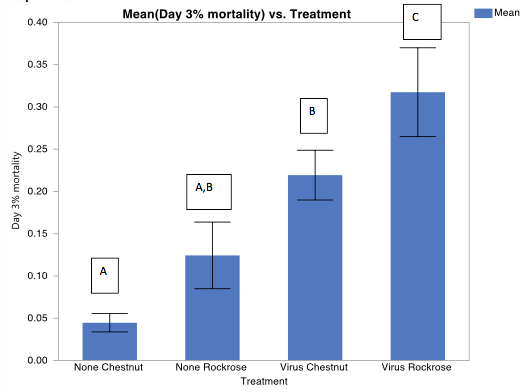
\includegraphics[width=0.8\textwidth]{Images/mortalityAll}
  \end{framed}
  \caption{Mortality rates between the four treatments. Each treatment contains 15 samples (cages).}
  \label{fig:mortalityAll}
\end{figure}

\begin{figure}[H]
\centering
  \begin{framed}
  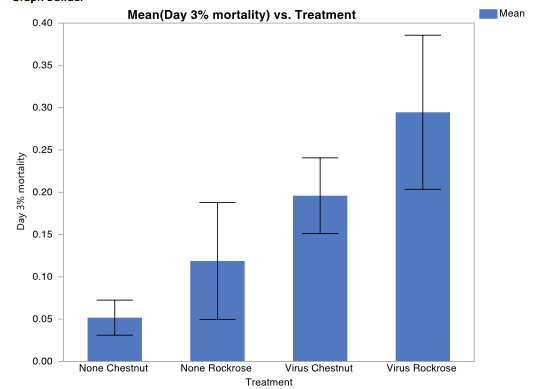
\includegraphics[width=0.8\textwidth]{Images/mortalityRNASeq}
  \end{framed}
  \caption{Mortality rates between the four treatments. Out of the original 15 samples (cages), each treatment here only contains the 6 samples (cages) that were used for RNA-sequencing.}
  \label{fig:mortalityRNASeq}
\end{figure}

\begin{figure}[H]
\centering
  \begin{framed}
  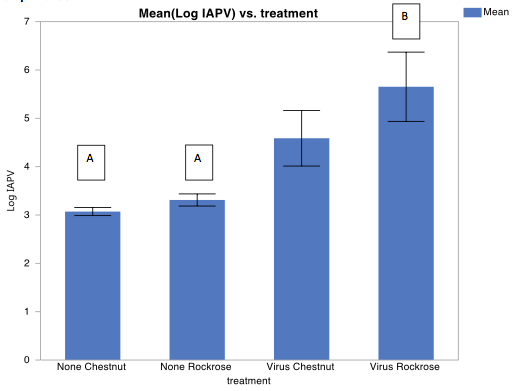
\includegraphics[width=0.8\textwidth]{Images/IAPVAll}
  \end{framed}
  \caption{IAPV titers between the four treatments. Each treatment contains 15 samples (cages).}
  \label{fig:IAPVAll}
\end{figure}

\begin{figure}[H]
\centering
  \begin{framed}
  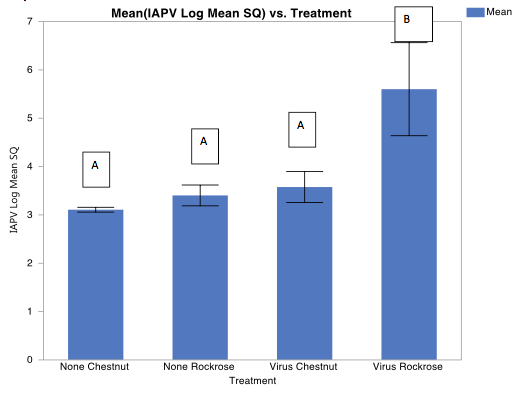
\includegraphics[width=0.8\textwidth]{Images/IAPVRNASeq}
  \end{framed}
  \caption{IAPV titers between the four treatments. Out of the original 15 samples (cages), each treatment here only contains the 6 samples (cages) that were used for RNA-sequencing.}
  \label{fig:IAPVRNASeq}
\end{figure}

Summary of what that paper found mortality, micronutrients
 We found that high quality diets (polyfloral pollen and high quality single-source pollen) have the potential to reduce mortality in the face of infection with Israeli acute paralysis virus (IAPV)
- There was a significant interaction between diet and virus infection on mortality, with associated differences in bee virus titers, suggesting good diets can help bees keep viral infection levels down





\section{Methods}





RNA-seq
RNA prep
Illumina sequencing at DNA facility
What version of genome mapped to
What mapping program did he use
What percent of reads mapped to the genome
Statistics (DESeq, EdgerR, visualizations, overlaps fisher, GO) 


\section{Results}


\section{Discussion}




% SYNTAX
%%%%%%%%%%%%%%%%%%%%%%%%%%%%%%%%%%%%%%%%%%%%%%%%%%%%%%%%%
%%%%%%%%%%%%%%%%%%%%%%%%%%%%%%%%%%%%%%%%%%%%%%%%%%%%%%%%%

%\ref{sec:ggenealogy}
% \code{ggparcoord}
% \Figure \ref{fig:porcupine}

% \begin{figure}[H]
% \centering
%     \begin{framed}
%     \includegraphics[width=0.8\textwidth]{porcupine}
%     \end{framed}
%     \caption{Three}
%     \label{fig:porcupine}
% \end{figure}

% \section{Literature review}
% \label{sec:litReview}

% \pkg{R} statistical programming language allows for tools to be distributed and modified at ease, encourages cross-platform collaboration, and provides a foundation for effective and aesthetic data visualization from the grammar of graphics. There are several useful \pkg{R} packages that offer tools for analyzing and visualizing genealogical datasets. Here, we introduce these packages, and emphasize the shortcomings for which our package \pkg{ggenealogy} brings to this collection of work.

%\clearpage

%\begin{enumerate}
%\item The data can be viewed at \url{http://shiny.soybase.org/CNV/}.
%\end{enumerate}

% \begin{tabular}{|p{2.6cm}|p{5.65cm}|p{5.65cm}|}
%  \hline
%  & \textbf{Drumming Treatment (D)} & \textbf{No Drumming Treatment (N)} \\ 
%  \hline
%  \textbf{Restricted} & \textbf{DR} & \textbf{NR} \\ 
%  \textbf{Nutrition (R)}& Predict most worker-like & Predict some worker-like \\
%  & gene expression & gene expression \\
%  \hline
%  \textbf{Unrestricted} & \textbf{DU} & \textbf{NU} \\ 
%  \textbf{Nutrition (U)} & Predict some worker-like & Predict least worker-like \\
%  & gene expression & gene expression \\
%  \hline
% \end{tabular}

\bibliography{chapter4}

\end{document}
